\subsection{RQ1: What software methodology are used in your project?}
\label{RQ1}
To find out the overall answer of this question, we report the following results:
\begin{itemize}
\item Software development methodologies (Q 6).
\item Requirements gathering (Q 7).
\item Most time consuming software development activities (Q 8).
\end{itemize}

\subsubsection{Methodologies}
The most-widely used model is Agile with usage rate of 40\%. The next widely-used model is scrum with usage rates of 30\%. The other methodologies has lower usage rates, namely: pair programming (13\%), Waterfall (8\%) etc. From the study we see that the most acceptable model that was regularly and always used is the agile model.
\begin{figure}[]
\centering
  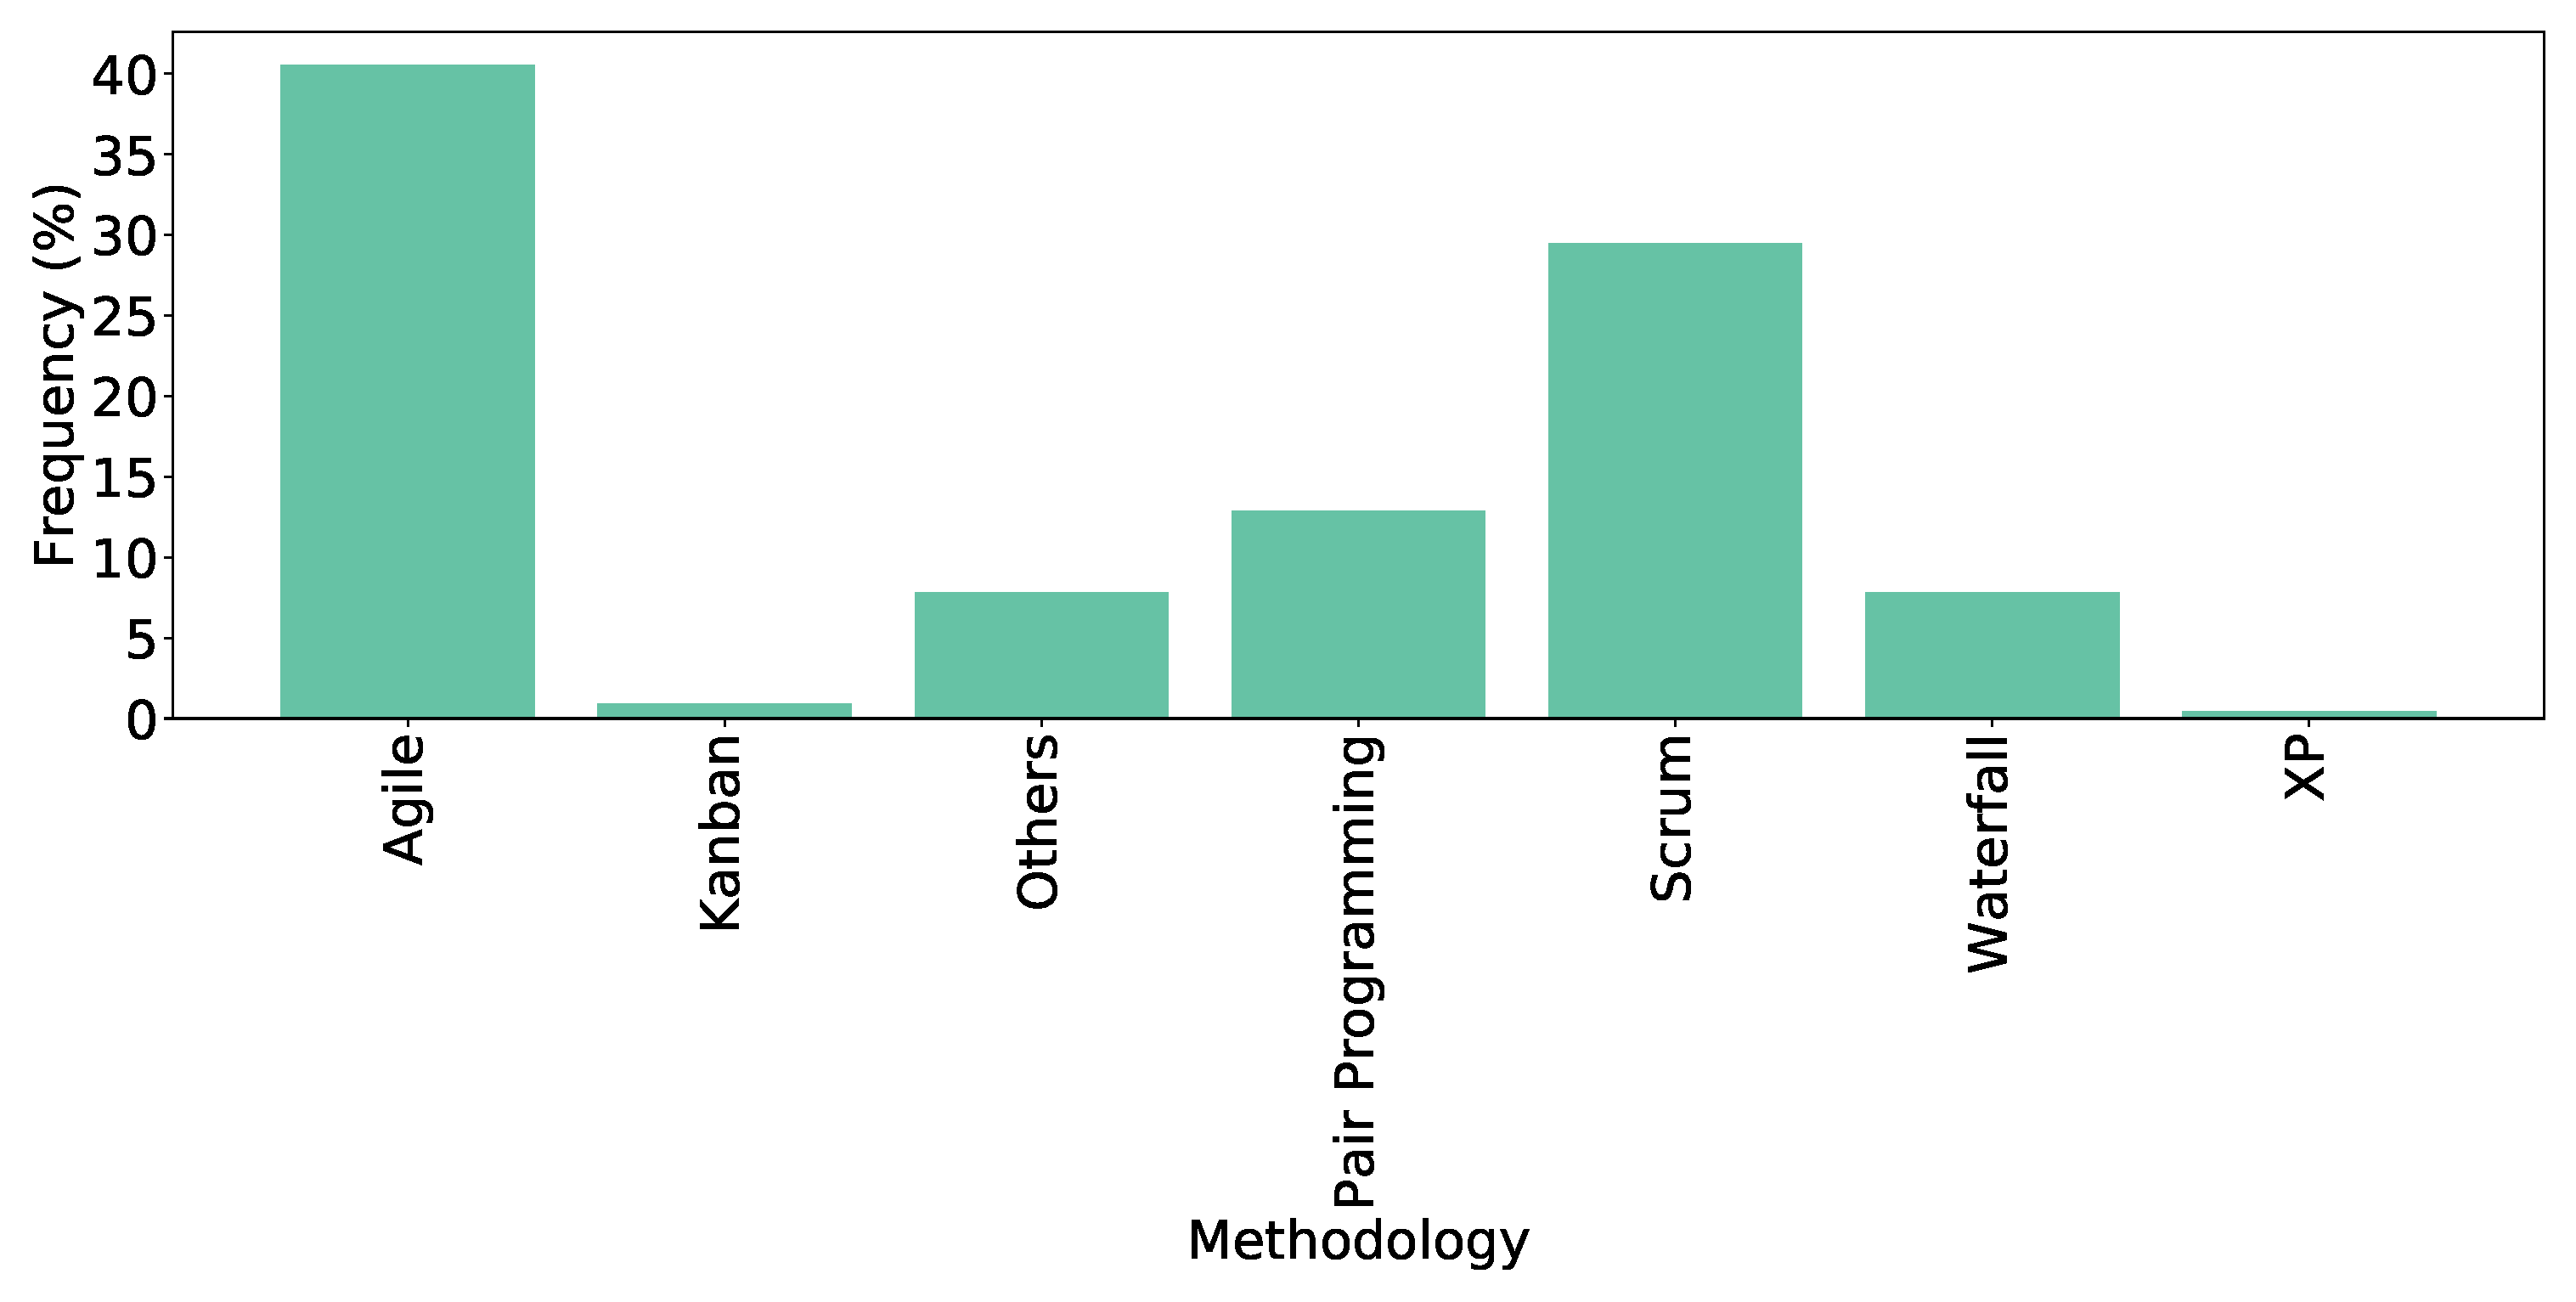
\includegraphics[width=0.8\textwidth]{Figures/Respondents_Methodology}
  \caption{Software development methodologies}
  \label{fig:methodologies}
\end{figure}

\subsubsection{Requirements Gathering}
The most critical activity that always arises during software development is the collecting requirement of the proposed system. According to \cref{fig:requirements}, using plain text (23\%) and story board(20\%) are the most widely used requirements gathering. The other requirements gathering usage rates are: Use case (18\%), GUI prototype (17\%), grooming session (15\%) etc. This is an important finding that requires further analysis for causes and to analyze the potential effects of not documenting requirements.
\begin{figure}[]
\centering
  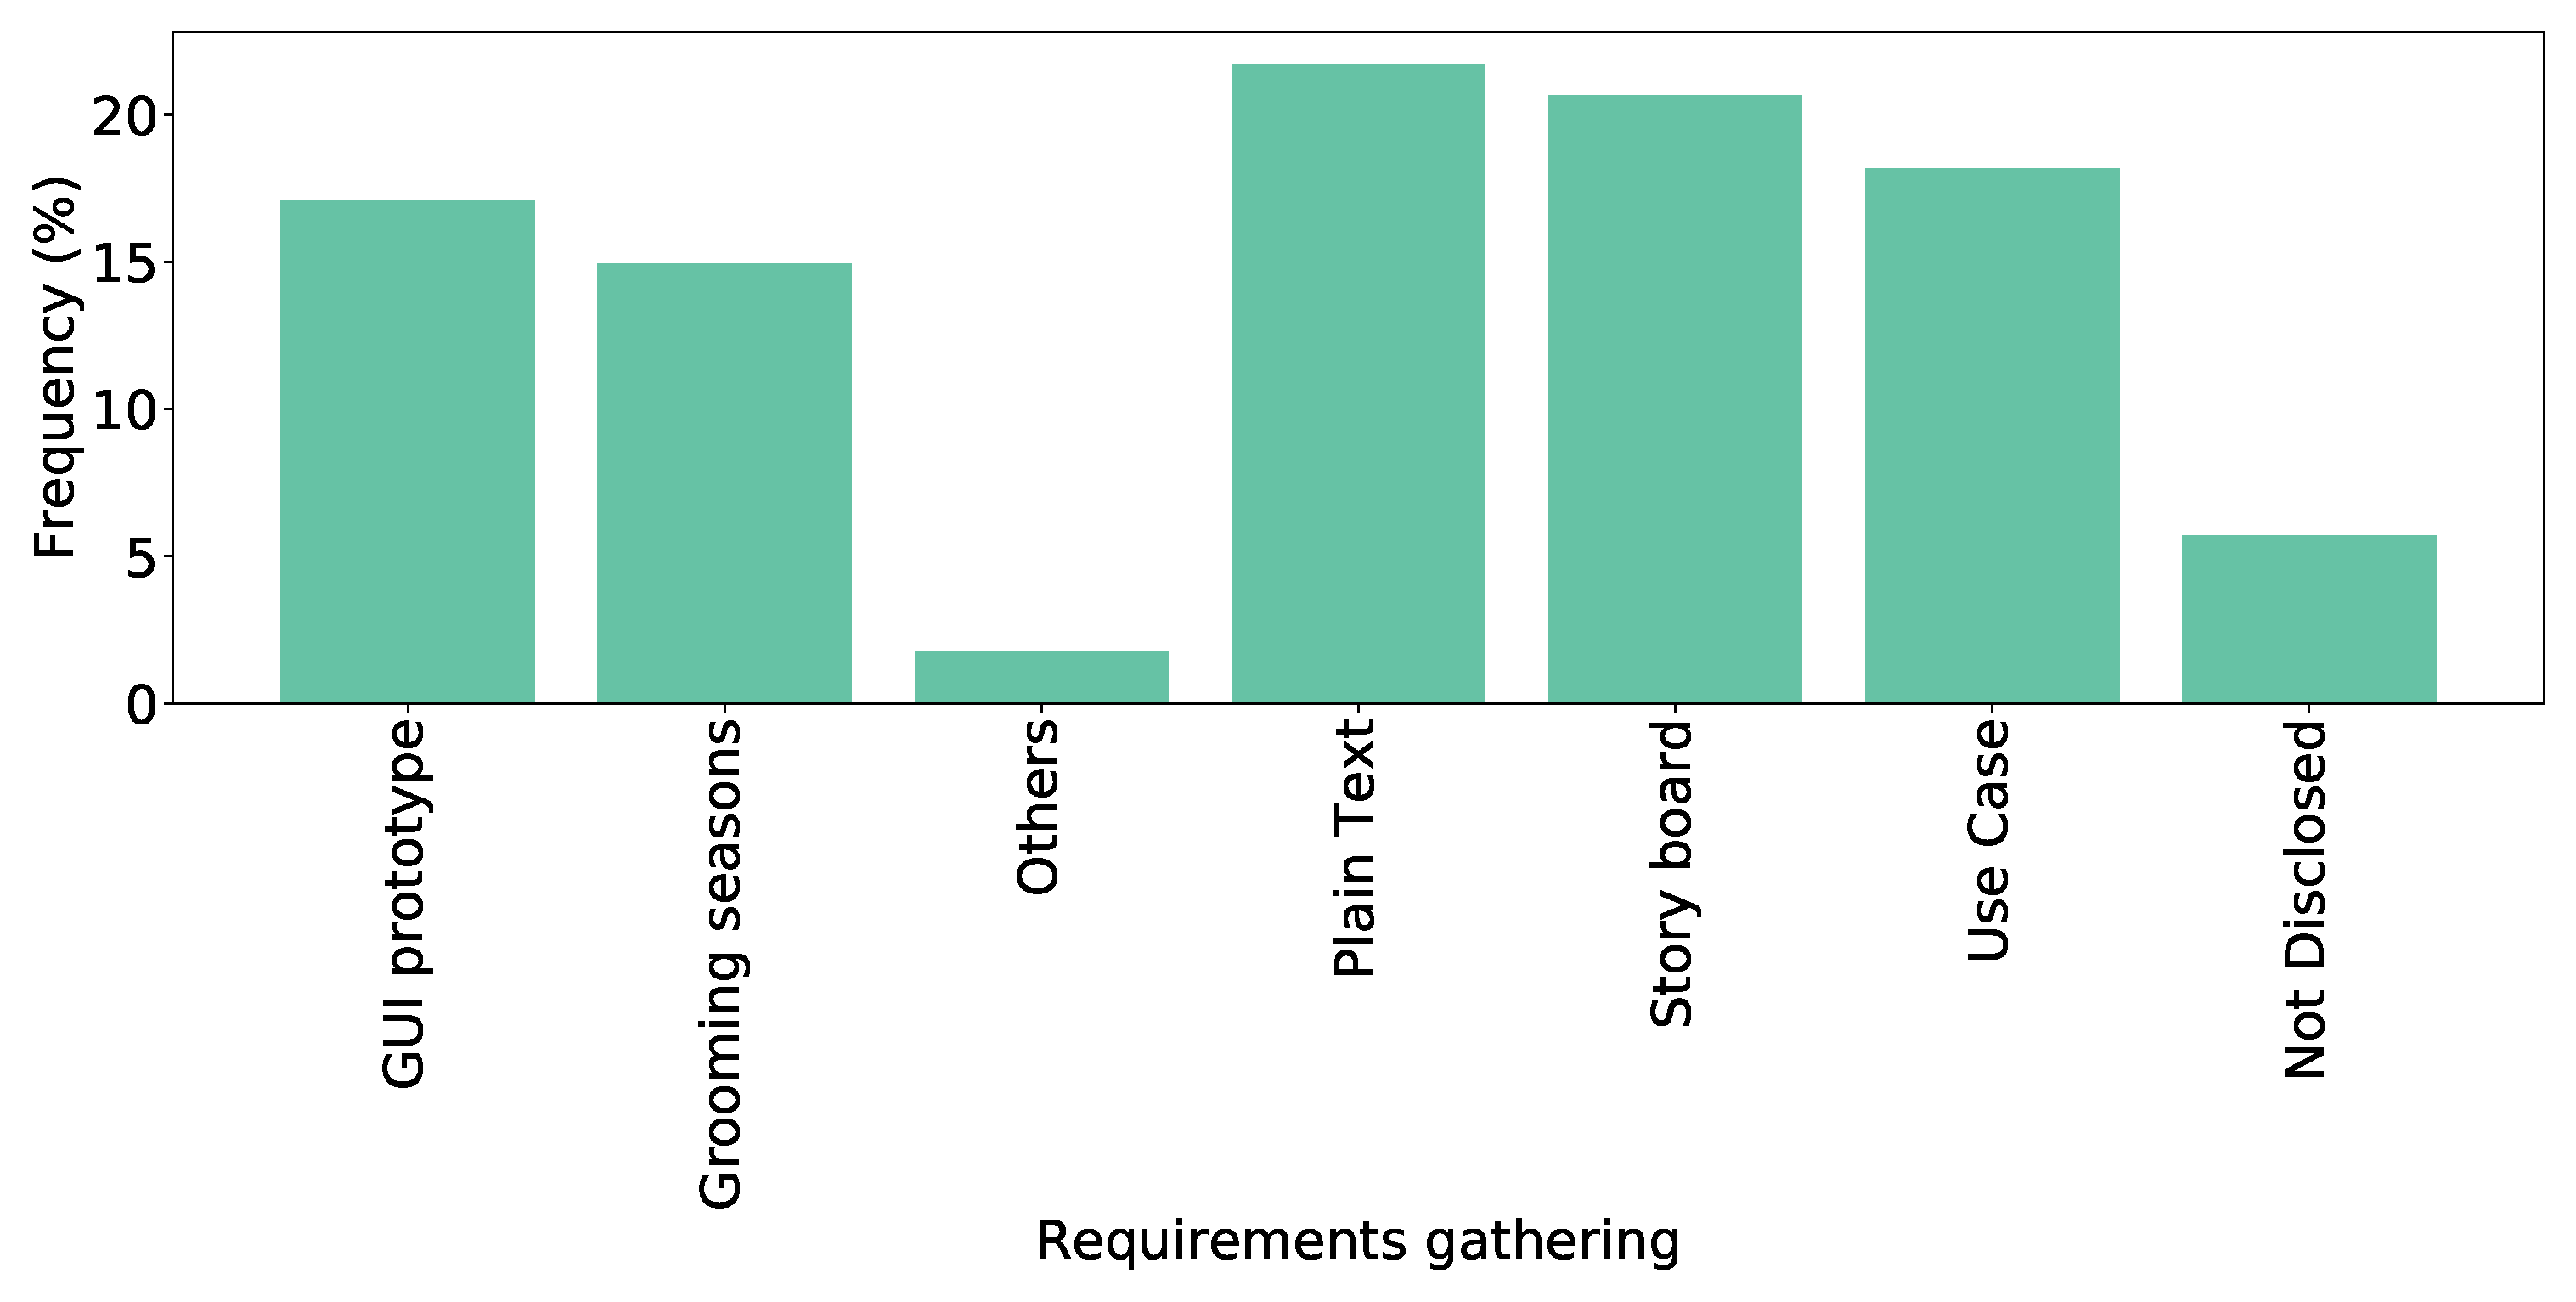
\includegraphics[width=0.8\textwidth]{Figures/Requirements_Gathering}
  \caption{Requirements gathering}
  \label{fig:requirements}
\end{figure}

\subsubsection{Development activities timeline}
In this section participants were asked about the most time consuming software developing activities they had spend. As we see in \cref{fig:activities}, most of the time spent in implementation stage (26\%) and requirement analysis stage (18\%) of the time. The other usages are: Program design (15\%), project planning (12.5\%), testing (8\%), maintenance (6\%) etc.
\begin{figure}[]
\centering
  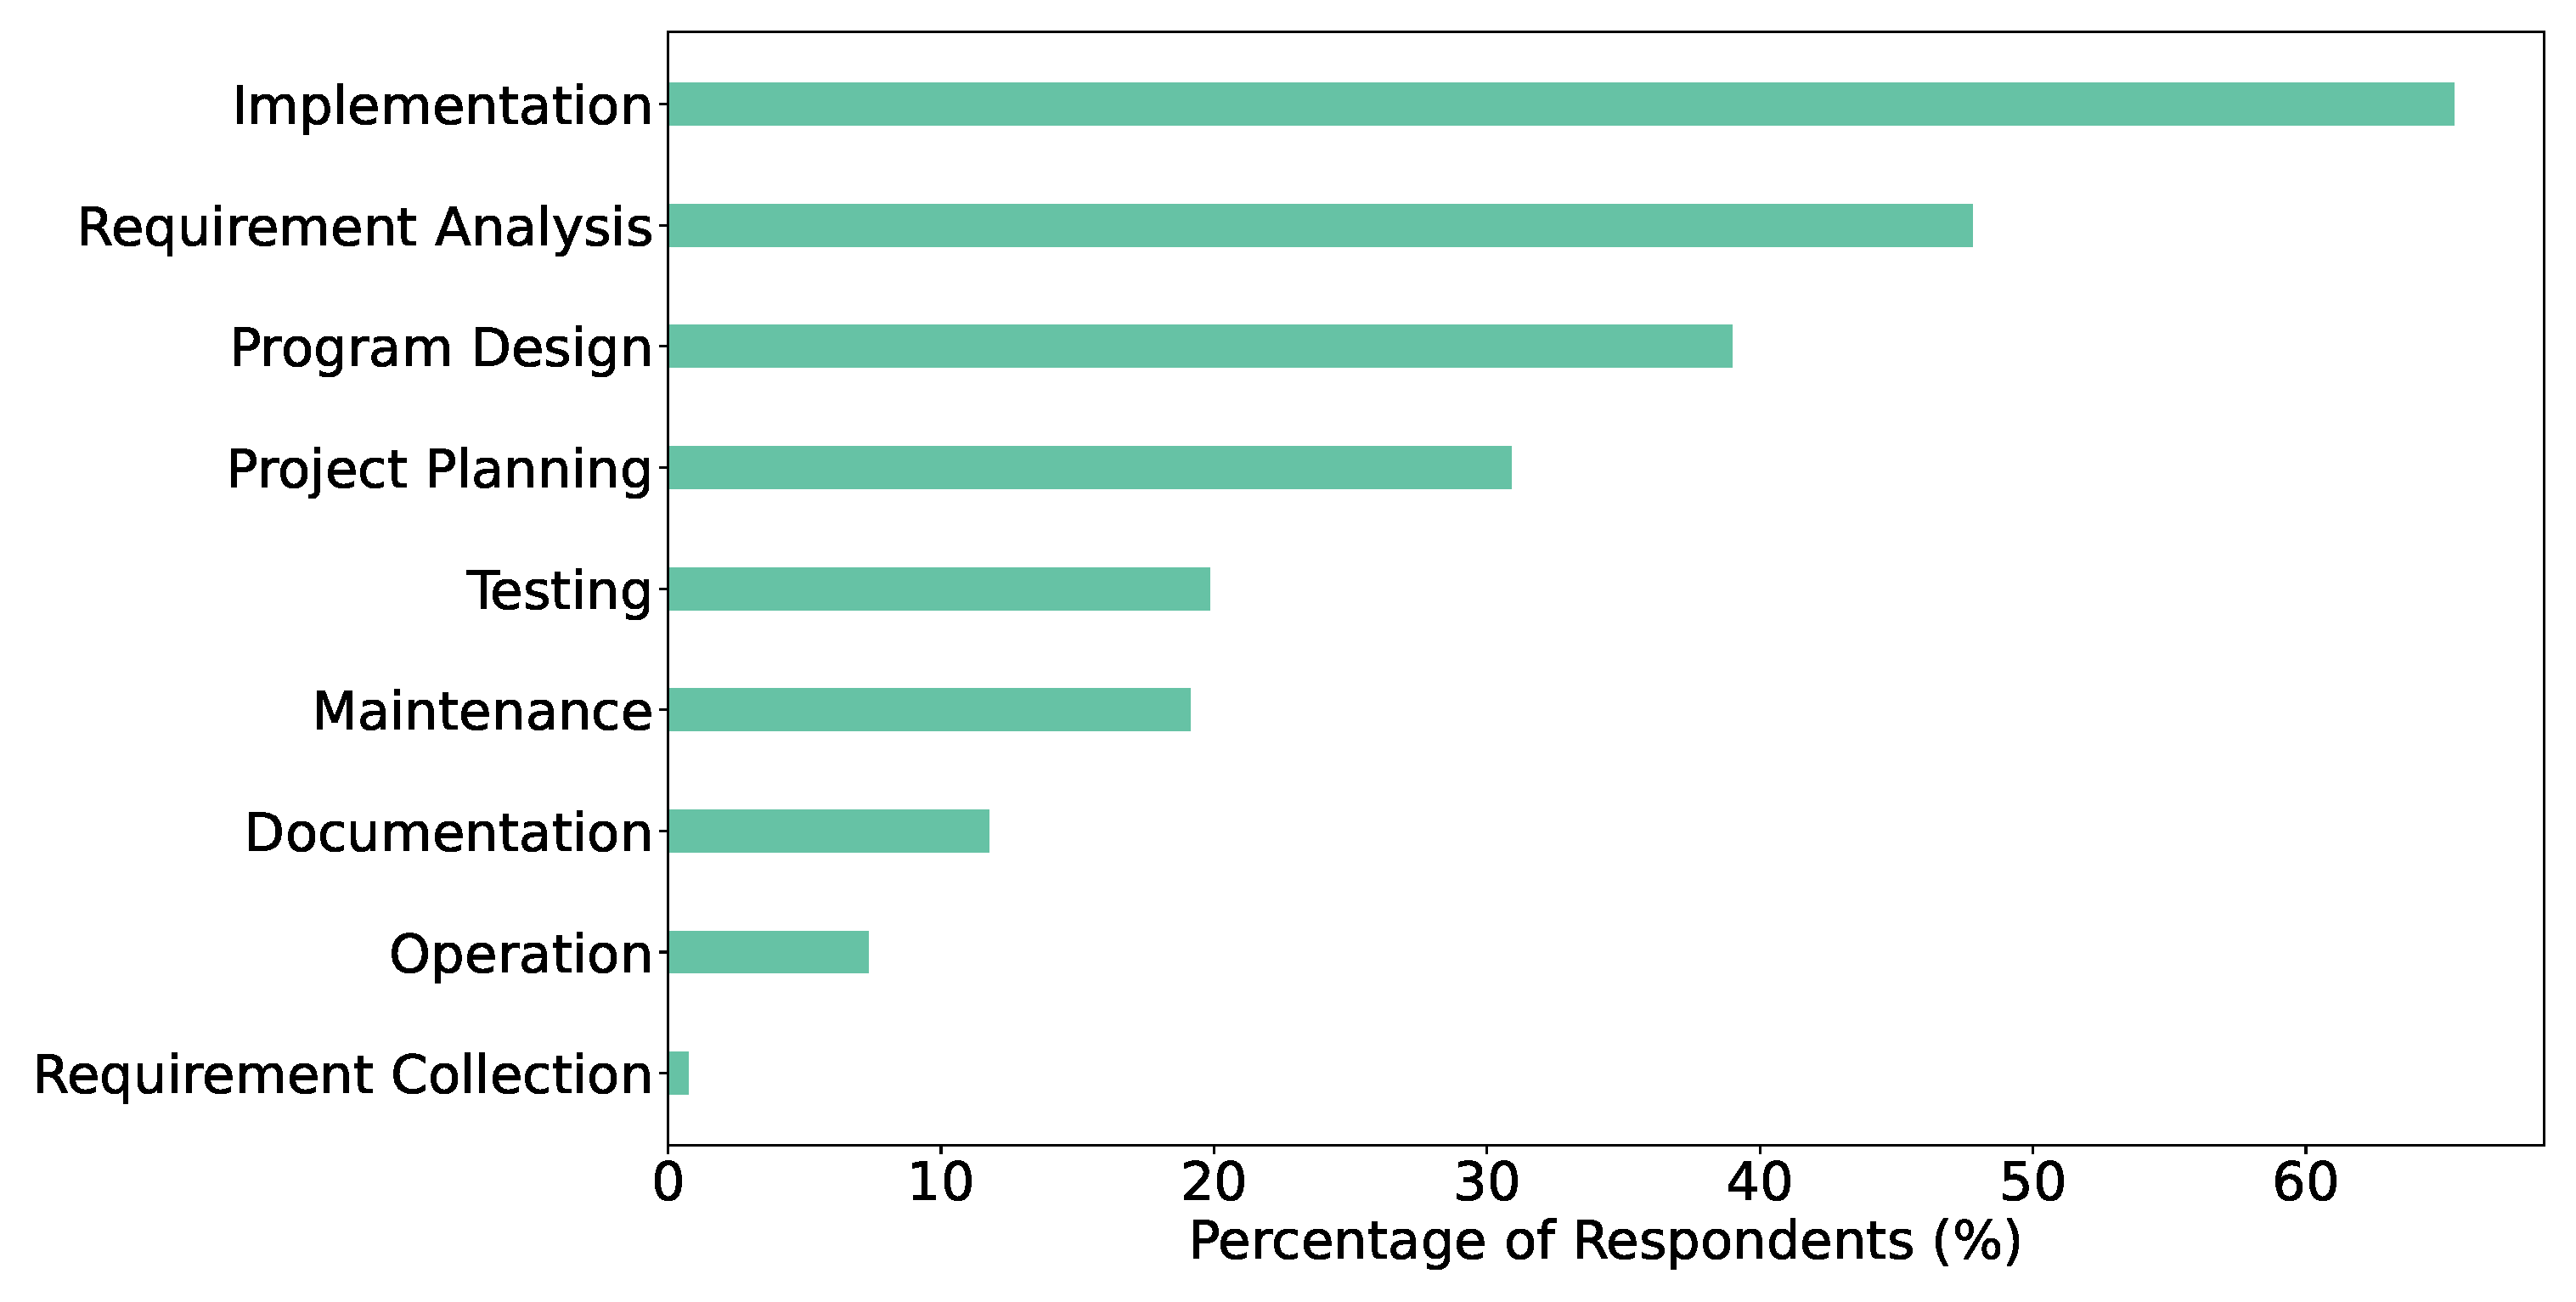
\includegraphics[width=0.8\textwidth]{Figures/Respondents_Activities}
  \caption{Software development activities}
  \label{fig:activities}
\end{figure}